\section*{Results}

\subsection*{Speedup}
\begin{frame*}
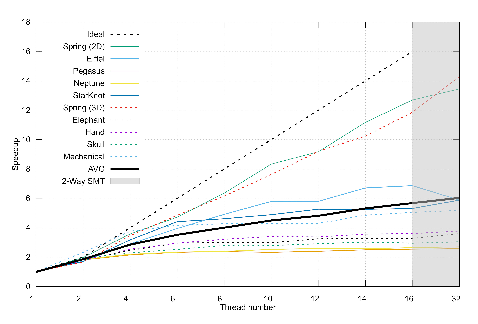
\includegraphics[width=\textwidth]{graph-speedup}
\end{frame*}

\subsection*{Number of tasks}
\begin{frame*}
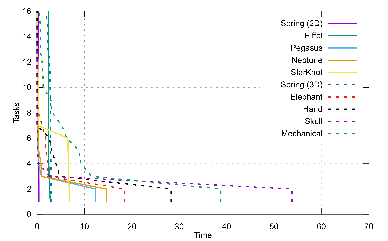
\includegraphics[width=\textwidth]{graph-tasks}
\end{frame*}

\subsection*{Conclusion}
\begin{frame*}
\begin{itemize}[<+->]
\item Parallel task-based algorithm for computing the augmented Reeb graph.
\item Improved laziness mechanism thanks to the locality of growths.
\item Dual sweep for improved parallel performance.
\item OpenMP/\cpluspluslogo{} implementation provided.
\end{itemize}
\begin{block}{What next?}<5->
\begin{itemize}
\item<6-> Number of tasks bounded by the number of leaves in the Reeb graph.
\item<7-> Number of independent local growths rapidly decreases to $2$.
\end{itemize}
\end{block}
\end{frame*}